\documentclass[letterpaper,11pt,twoside]{article}
\usepackage[utf8]{inputenc}
\usepackage{amsmath,amsfonts,amssymb,amsthm,latexsym}
\usepackage[spanish,es-noshorthands]{babel}
\usepackage[T1]{fontenc}
\usepackage{lmodern}
\usepackage{graphicx,hyperref}
\usepackage{tikz,pgf}
\usepackage{multicol}
\usepackage{fancyhdr}
\usepackage[height=9.5in,width=7in]{geometry}
\usepackage{fancyhdr}
\pagestyle{fancy}
\fancyhead[LE]{
\includegraphics[height=12pt]{Images/logo-colegio.png} Geometría $6^{\circ}$}
\fancyhead[RE]{}
\fancyhead[RO]{\textit{Germ\'an Avenda\~no Ram\'irez, Lic. U.D., M.Sc. U.N.}}
\fancyhead[LO]{}

\author{Germ\'an Avenda\~no Ram\'irez, Lic. U.D., M.Sc. U.N.}
\title{\begin{minipage}{.2\textwidth}

\includegraphics[height=1.75cm]{Images/logo-colegio.png}\end{minipage}
\begin{minipage}{.55\textwidth}
\begin{center}
Taller 04, Elementos gráficos\\
Geometría $6^{\circ}$
\end{center}
\end{minipage}\hfill
\begin{minipage}{.2\textwidth}

\includegraphics[height=1.75cm]{Images/logo-sed.png} 
\end{minipage}}
\date{}
\thispagestyle{plain}
\begin{document}
\maketitle
Nombre: \hrulefill Curso: \underline{603} Fecha: \underline{\hspace*{2.5cm}}
\begin{multicols}{2}
\section*{Aprendo algo nuevo}
\begin{itemize}
\item Comencemos entonces, por diferenciar las figuras
abiertas y las cerradas.
\end{itemize}
\begin{center}
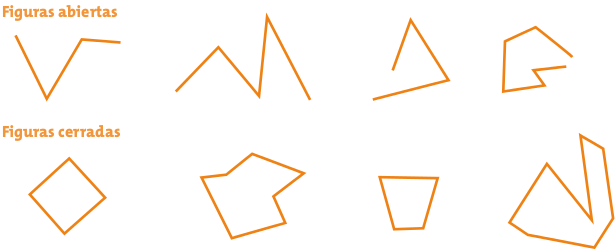
\includegraphics[scale=.4]{Images/Fig_abiertas_cerradas.png} 
\end{center}
Escribe algunas características que identifiques en cada uno
de los grupos de líneas, ya sean abiertas o cerradas.
\begin{itemize}
\item ¿En qué grupo incluirías el esquema que elaboró
Guillermo, según la situación planteada en la primera
página de esta guía?
\item Revisando nuevamente la situación, Guillermo plantea
un punto de partida (el corral de las vacas), que coincide
con el punto final. Por lo tanto, el recorrido descrito por
Guillermo corresponde a una línea poligonal cerrada.
\end{itemize}
\begin{center}
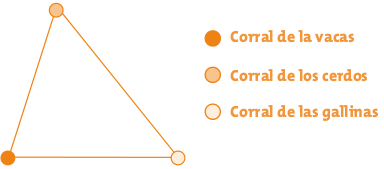
\includegraphics[scale=.55]{Images/corrales.png}
\end{center}
Se denomina línea poligonal al conjunto ordenado de segmentos tales que, el extremo de uno de ellos coincide con
el origen del segmento que le sigue. Un polígono está con-
formado por una línea poligonal cerrada.

La palabra polígono está formada por dos voces de origen griego: "polys": muchos y "gonía": ángulos; por lo tanto,
es una figura con muchos ángulos.
\begin{itemize}
\item ¿Cuántos ángulos identificas en el dibujo elaborado por
Guillermo?
\item ¿Qué tiene en común este número con el número de
lados o segmentos?
\end{itemize}
Guillermo se pregunta qué figura se formaría si en lugar
de ir a tres puntos diferentes tuviera que desplazarse consecutivamente por cuatro, cinco, o más puntos. Dibuja en
tu cuaderno los esquemas correspondientes. Escribe cuántos
lados tiene cada polígono.
\begin{center}
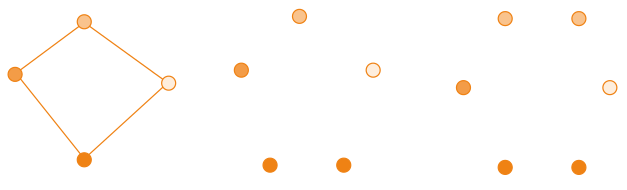
\includegraphics[scale=.4]{Images/poligonos.png} 
\end{center} 
\section*{Ejercito lo aprendido}
Elabora la tabla en tu cuaderno y registra el número de lados,
ángulos y vértices que tiene cada polígono. Ten en cuenta que
en la tabla se presenta la clasificación de polígonos según sus
lados.
\begin{center}
\begin{tabular}{|c|c|c|c|}
\hline 
Polígono & Lados & Vértices & Ángulos \\ 
\hline 
Triángulo \tikz \filldraw[gray] (0,0)--(1,0)--(1,1)--cycle; &  &  &  \\ 
\hline 
Cuadrilátero \tikz \filldraw[gray] (0,0) rectangle (1.2,1); &  &  &  \\ 
\hline 
Pentágono 
\includegraphics[scale=.6]{Images/pentagono.png}   &  &  &  \\ 
\hline 
Hexágono 
\includegraphics[scale=.6]{Images/hexagono.png} &  &  &  \\ 
\hline 
Heptágono 
\includegraphics[scale=.6]{Images/heptagono.png} &  &  &  \\ 
\hline 
Octágono 
\includegraphics[scale=.6]{Images/octagono.png}  &  &  &  \\ 
\hline 
\end{tabular} 
\end{center}
\begin{enumerate}
\item ¿Qué tienen en común los polígonos qué se presentaron en
la tabla anterior?
\item Dibuja otros polígonos que tengan las mismas
características de los que se presentaron en la tabla, pero
que tengan diferente forma.
\end{enumerate}
\end{multicols}
\end{document}
